\section{Evaluation}
\label{sec:evaluation}

Inference-time trustworthiness methods intervene after model training to shape LLM behavior under deployment constraints. As these interventions differ a lot in where and how they act, such as in prompts, logits, activations, external filters, or the system workflow, evaluation cannot be unified by one benchmark or one metric family. Although foundational benchmarks such as TrustGPT~\citep{huang2023trustgpt} and dynamic evaluation toolkits such as TrustEval~\citep{wang2025trusteval} provide valuable unified views over multiple trustworthiness dimensions, they were not designed to isolate the runtime-specific properties introduced by inference-time controls. We therefore adopt a meta-axis evaluation view on the inference-time evaluation. The goal is to capture deployment-relevant properties that arise specifically from runtime trustworthiness. In practice, such enforcement is shaped by latency, cost, and integration constraints. Each axis highlights a distinct evaluation question, and while the axes are conceptually unique, they can overlap in practice:

\begin{figure*}[htbp]
  \centering
  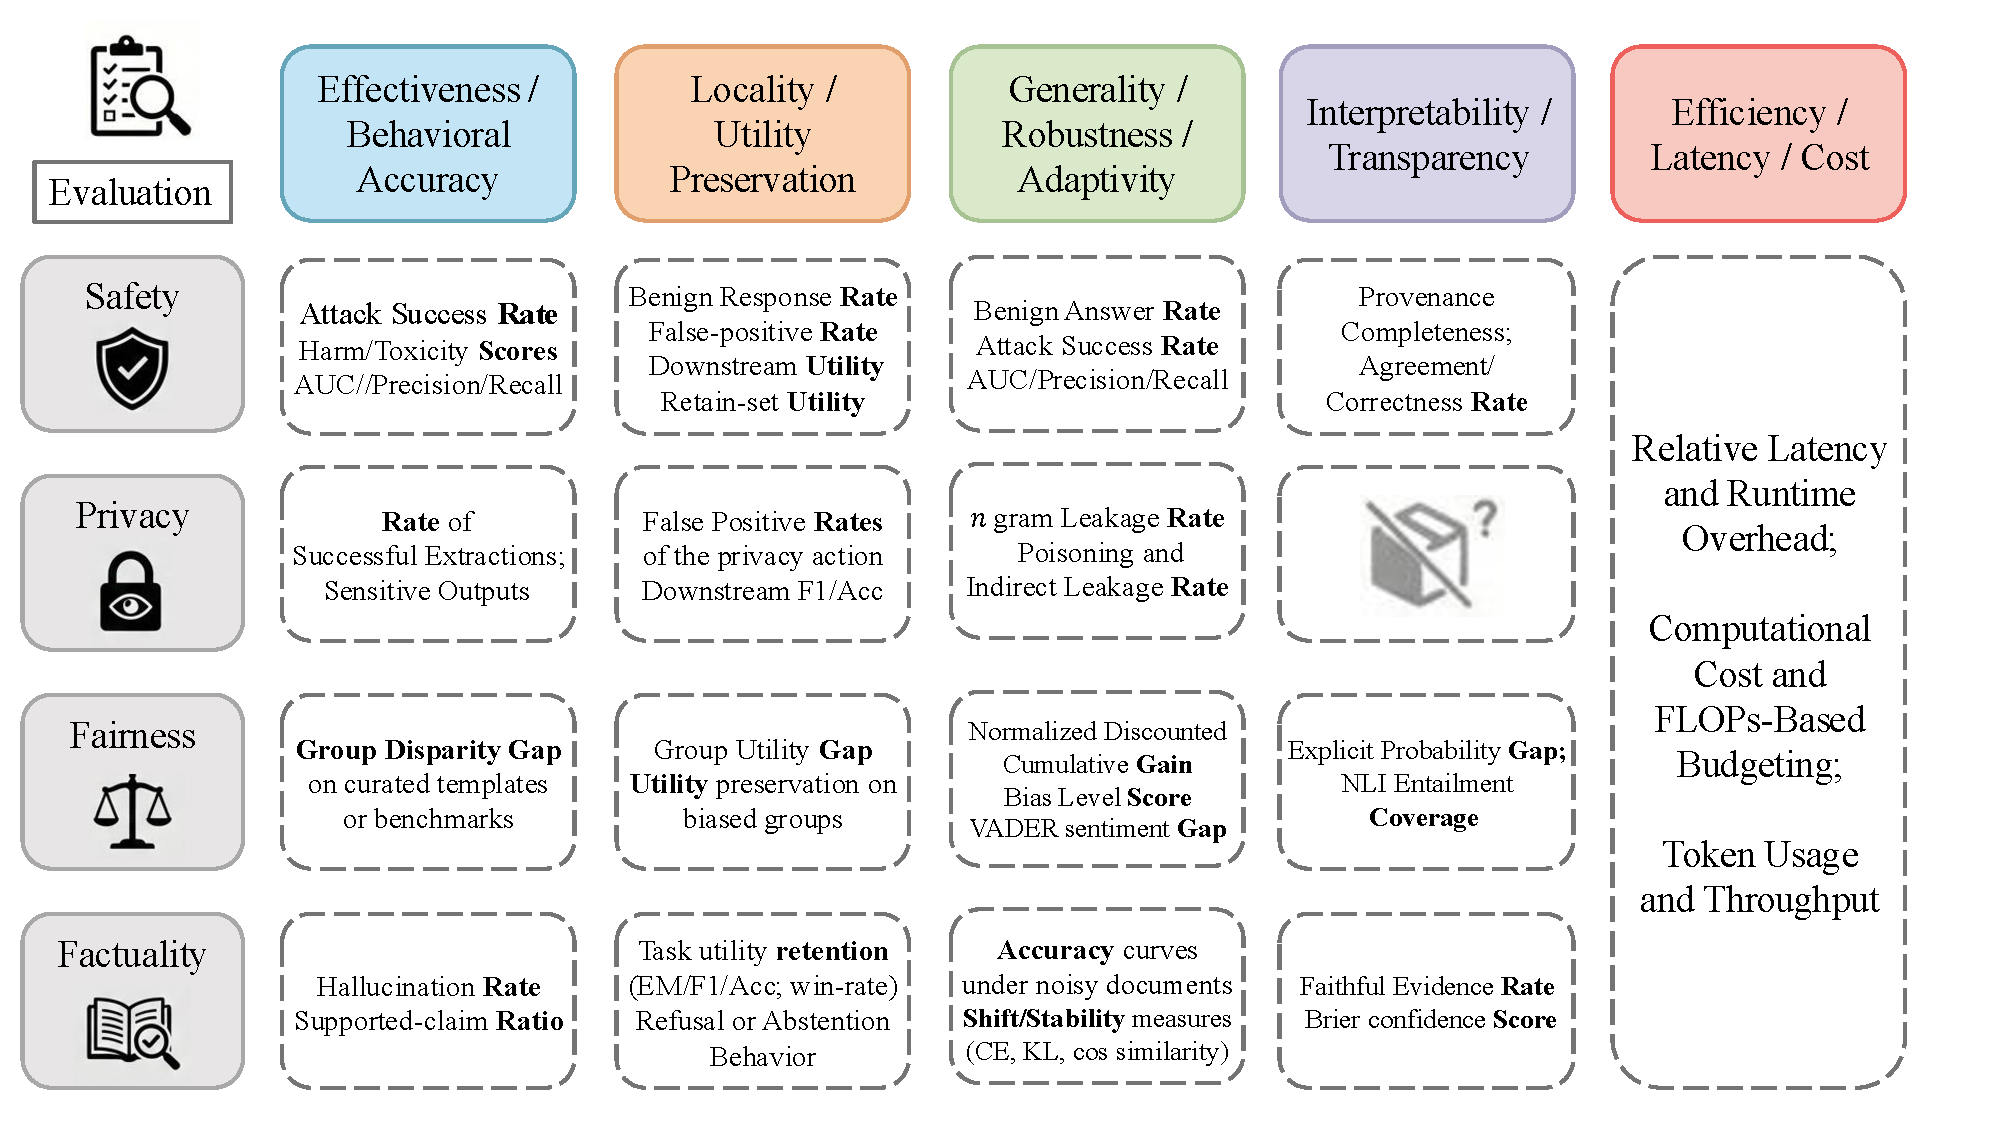
\includegraphics[width=0.9\linewidth]{figures/method/evaluations.pdf}
  \caption{A meta-axis evaluation framework for inference-time trustworthiness methods. Rows correspond to four trustworthiness dimensions (Safety, Privacy, Fairness, Factuality), and columns represent five complementary evaluation axes (Effectiveness, Locality, Generality, Interpretability, Efficiency). Each cell lists representative metrics specific to the dimension--axis intersection, highlighting the multi-faceted nature of deployment-time evaluation.}
  \label{fig:evaluation}
\end{figure*}

\begin{itemize}
\item \textbf{Effectiveness / Behavioral Accuracy}: To what extent does the inference-time mechanism reliably enforce the intended behavioral constraints, and under what conditions does it fail?
\item \textbf{Locality / Utility Preservation}: To what extent are the intervention effects localized to the targeted behaviors while preserving general task performance and user utility?
\item \textbf{Generality / Robustness / Adaptivity}: How well does the mechanism generalize across tasks, domains, and input distributions, and how robust is it to distributional shifts?
\item \textbf{Efficiency / Latency / Cost}: What additional runtime overhead does the mechanism introduce in terms of latency, compute, memory, or token usage?
\item \textbf{Interpretability / Transparency}: To what extent are the mechanism’s actions, triggers, and decision rationales transparent to human auditors or downstream systems?
\end{itemize}

Although these axes separate different deployment concerns, they often trade off against one another. 
% For example, a guardrail detector may score highly on effectiveness, such as achieving a high AUC, yet still fail on locality by excessively blocking benign content. Similarly, a method can succeed on safety under standard conditions but fail on robustness when it is bypassed by prompt injection.
Building on this framing, this section organizes evaluation along the axes above and surveys representative metrics, across four categories: Safety, Privacy, Fairness, and Factuality.

\subsection{Effectiveness / Behavioral Accuracy}
Effectiveness / Behavioral Accuracy evaluates whether an inference-time mechanism $\mathcal{M}$ changes model behavior in the intended direction on a target evaluation distribution. Consider an LLM that produces an output $Y_{\mathcal{M}}(x)$ for an input $x \sim \mathcal{D}$ under $\mathcal{M}$. Effectiveness asks whether $\mathcal{M}$ increases the likelihood of desired trust-aligned behavior and decreases the likelihood of undesired behavior:
\[
\text{Effectiveness}(\mathcal{M}) \propto
\mathbb{E}_{x \sim \mathcal{D}}
\Big[
\mathbf{1}\{Y_{\mathcal{M}}(x)\in \mathcal{Y}_{\text{desired}}\}
-
\mathbf{1}\{Y_{\mathcal{M}}(x)\in \mathcal{Y}_{\text{undesired}}\}
\Big].
\]
In inference-time settings, this axis primarily measures the runtime behavior induced by a plug-in control layer, such as refusal, redaction, constrained decoding, evidence grounding, or verification. However, Effectiveness alone does not tell whether improvements come from overly broad suppression of benign behavior, from brittle operating thresholds, or from masking the underlying capability. These trade-offs motivate complementary axes such as Locality (utility and over-refusal), Robustness (bypassability and shift), Efficiency (latency/cost), and Interpretability (auditability).

\subsubsection{Rate-Based Metrics}
Rate-based metrics capture how often undesired behavior still occurs at inference time, and are the most prevalent family across all trustworthiness categories. In safety, jailbreak success rate measures whether an adversarial prompt elicits a harmful response from the model, unsafe completion rate tracks the overall proportion of harmful outputs across all queries, and the complementary defense success rate captures how often the mechanism successfully blocks such outputs. Risk-score formulations take a continuous toxicity or harm score assigned to each output instead of a binary attack outcome and report the fraction exceeding a predefined threshold~\citep{kumar2024certifying, Xu2024SafeDecodingDA, Huang2024SafeAlignerSA, chen2025safeptr, deng2025guard, hasan2024pruning, fan2025peerguarddefendingmultiagentsystems, yan2025dual}. In privacy, extraction success rate captures whether an attacker can recover memorized or sensitive text from model outputs, while disclosure rate measures how often outputs contain personally identifying or otherwise private information across a broader query distribution~\citep{pawelczyk2023context, Borec2024TheUI, Wang2025PrivacyAwareDM, zou2025poisonedrag}. In factuality, hallucination rate counts the proportion of outputs that are unsupported or factually incorrect, groundedness rate measures the fraction of claims in a response that are explicitly supported by retrieved or provided evidence, and edit success rate verifies whether a targeted fact has been correctly updated following a knowledge editing intervention~\citep{dhuliawala2024chain, asai2024self, zhou2024metacognitive, meng2022locating, meng2022memit}.

\subsubsection{Classifier-Style Metrics}
Classifier-style metrics treat the inference-time intervention as an explicit detection task and evaluate how well the mechanism separates harmful, private, or hallucinated outputs from benign ones. Rather than reporting a single operating point, metrics such as AUC and AUPRC summarize performance across all possible decision thresholds, while Precision, Recall, and F1 show the trade-off between false positives and false negatives at a chosen threshold. These metrics are important when the intervention involves a learned or rule-based classifier, such as a safety guardrail or hallucination detector, where threshold calibration governs deployment behavior. They appear across safety guardrails~\citep{Padhi2024GraniteG, Chi2024LlamaG3, Kumar2025PolyGuardAM, Liu2025GuardReasonerTR}, privacy membership-inference evaluations~\citep{zou2025poisonedrag, nakka2025piijailbreaking}, and factuality hallucination detection~\citep{asai2024self, zhou2024metacognitive}.

\subsubsection{Group-Disparity Metrics}
Group-disparity metrics quantify fairness effectiveness by comparing outcomes across demographic groups, capturing whether a mechanism treats different populations equitably. Bias scores on curated benchmarks measure stereotyping or differential toxicity for specific groups, worst-group performance identifies the most disadvantaged subpopulation, and disparity gaps capture the absolute difference in an outcome metric such as toxicity, error rate, or refusal rate between two groups. Together, these metrics reveal whether a fairness intervention reduces imbalance in model behavior or merely shifts it. They are reported across prompt-based interventions~\citep{dwivedi2023breaking, huang2024bias, kamruzzaman2024prompting}, fairness-aware retrieval~\citep{chen2024spica, shrestha2024fairrag}, and pruning methods that target bias-related internal structure~\citep{cai2024locating, zayed2024fairness, ma2025breaking}.

\subsubsection{Task-Performance Metrics}
Task-performance metrics such as exact match, F1, and accuracy measure whether trustworthiness gains come at the cost of general capability, serving as a sanity check on standard benchmarks. They are widely reported among representation or context engineering evaluations to confirm that they do not disrupt unrelated competencies~\citep{li2023iti, bayat2024enhanced, wang2024act, meng2022locating}, and also appear in multimodal hallucination settings~\citep{Park2024ConVisCD, Yuan2024HELPDMH}.

% Across all four categories, a low failure rate does not imply a better system if it results from an overly conservative operating point that suppresses benign requests, and task-accuracy gains can be confounded by format changes or benchmark saturation. Effectiveness metrics should therefore always be interpreted alongside Locality, Robustness, and Interpretability evaluations.

\subsection{Locality / Utility Preservation}
Locality / Utility Preservation evaluates whether an inference-time mechanism $\mathcal{M}$ limits its behavioral changes to the intended outputs while preserving user utility. Unlike training-time alignment, inference-time controls are typically implemented as plug-in layers. As a result, the locality failure mode is behavioral spillover, in which the system becomes safer by being less helpful, issuing more refusals, or providing less information. Formally, let $\mathcal{D}_{\text{tgt}}$ denote the targeted distribution (e.g., harmful or sensitive prompts) and $\mathcal{D}_{\text{benign}}$ denote benign traffic. A generic utility retention view is:
\[
\Delta U_{\text{benign}}(\mathcal{M})
=
\mathbb{E}_{x\sim \mathcal{D}_{\text{benign}}}\!\left[u\!\left(Y_{\mathcal{M}}(x)\right) - u\!\left(Y(x)\right)\right],
\]
where $u(\cdot)$ can be task accuracy (EM/F1/Acc), LLM-as-judge helpfulness, or win-rate. In inference-time deployment, locality is coupled to thresholding and pipeline composition. When multiple strategies are combined, such as guardrails and decoding, they can amplify suppression of benign outputs even if each component appears acceptable in isolation.


\subsubsection{False-Positive and Over-Refusal Rate Metrics}
These metrics capture whether a mechanism incorrectly suppresses or refuses inputs it was not designed to target. In safety, benign response rate measures how often the defense leaves safe prompts unaffected, and is usually reported alongside attack success rate to confirm that refusal gains are not simply the result of refusing more broadly~\citep{kumar2024certifying, cao2024defending, ji2024defending, zhou2024defending}. In guardrail systems, false-positive rate and benign blocking rate capture how often clean inputs are incorrectly filtered or routed. These summarize the trade-off between blocking harmful content and passing benign traffic~\citep{Padhi2024GraniteG, Chi2024LlamaG3, Kumar2025PolyGuardAM, Liu2025GuardReasonerTR}. In multi-agent defenses, false alarm rates on clean interactions are essential because a monitoring agent that incorrectly flags benign exchanges can suppress the entire downstream workflow~\citep{fan2025peerguarddefendingmultiagentsystems, asad2025reddebatesaferresponsesmultiagent}. In privacy, false positives of the privacy action through blocking harmless queries, measure damage on non-sensitive content~\citep{pawelczyk2023context, Wang2025PrivacyAwareDM}. In fairness, refusal disparity measures the absolute difference in refusal rate between demographic groups under the intervention, capturing whether the mechanism disproportionately suppresses responses for certain groups rather than improving equitable helpfulness~\citep{dwivedi2023breaking, huang2024bias, kamruzzaman2024prompting}.

\subsubsection{Utility Retention Metrics}
Utility retention metrics measure whether general task performance is preserved on non-targeted inputs after the intervention. Common metrics include exact match, F1, and accuracy on held-out benchmarks, MT-Bench scores, instruction-following rates, LLM-as-judge helpfulness, and win-rate. In safety, these are reported for decoding, representation engineering, pruning, and unlearning interventions to confirm that modifications do not distort normal generation quality~\citep{Xu2024SafeDecodingDA, Arditi2024SingleDirection, chen2025safeptr, hasan2024pruning, deng2025guard, zhang2024theft}. In privacy, downstream task accuracy on non-sensitive queries confirms that filtering or constrained generation does not broadly reduce answer quality~\citep{Borec2024TheUI, zou2025poisonedrag}. In fairness, per-group utility retention tracks whether task success is preserved equitably across demographic groups, ensuring bias reduction is not obtained by broadly degrading helpfulness for any subpopulation~\citep{shrestha2024fairrag, cai2024locating, zayed2024fairness, ma2025breaking}. In factuality, retain-set task utility on benign factual QA is reported alongside hallucination reductions~\citep{dhuliawala2024chain, li2023iti, asai2024self, zhou2024metacognitive}.

\subsection{Generality / Robustness / Adaptivity}
Generality / Robustness / Adaptivity evaluate whether an inference time mechanism $\mathcal{M}$ keeps its intended effect when inputs, tasks, or attackers change at deployment. This axis is not about a single test set. It is about performance over a family of conditions, which is likely out-of-distribution. Let $\{\mathcal{D}_k\}_{k=1}^K$ be test distributions and let $s_k(\mathcal{M})$ be a score on $\mathcal{D}_k$. A common summary reports both the average and the worst case:
\[
s_{\mathrm{avg}}(\mathcal{M})=\frac{1}{K}\sum_{k=1}^K s_k(\mathcal{M}),
\qquad
s_{\min}(\mathcal{M})=\min_{k\in[K]} s_k(\mathcal{M}).
\]
% In inference-time settings, $s_{\min}$ is often more critical for deployment because the system must handle rare but high-risk inputs.

\subsubsection{Worst-Case and Cross-Distribution Rate Metrics}
These metrics summarize how a mechanism's core effectiveness signal holds up across multiple conditions rather than a single fixed distribution. In safety, attack success rate and benign answering rate are reported across multiple jailbreak families and prompt styles, with worst-case values serving as the primary robustness summary. Sensitivity to threshold changes is captured by reporting deltas when guard strength varies~\citep{kumar2024certifying, cao2024defending, zhou2024defending}. Decoding and representation engineering methods report harmful score and safety score under stronger or more diverse attacks. Tracking utility accuracy on task suites to confirm that robustness gains do not come at the cost of normal performance~\citep{Xu2024SafeDecodingDA, Wang2024InferAligner, deng2025guard}. In privacy, attack success rate is reported across multiple attack types and privacy budgets to capture how leakage behavior changes as the adversary changes. N-gram leakage rate measures whether the control generalizes beyond exact span matches to broader overlap with sensitive content~\citep{tong2025inferdpt, chaudhari2024phantom}. In fairness, bias scores and stereotype index are reported across demographic categories, topics, and occupations to evaluate whether bias reduction holds beyond a fixed template. Fairness violation rates are tracked alongside utility metrics such as NDCG~\citep{kamruzzaman2024prompting, dwivedi2023breaking, huang2024bias}. In factuality, accuracy and F1 are reported across cross-domain splits to test whether robustness comes from better evidence selection rather than longer contexts~\citep{wan2024dell, dhuliawala2024chain, zhou2024metacognitive, asai2024self}.

\subsubsection{Classifier-Style Metrics Across Domains and Languages}
When the intervention involves an explicit detector or classifier, robustness is evaluated by reporting precision, recall, F1, AUC, and AUPRC across multiple benchmarks, domains, and languages. In safety, guardrails and multi-agent systems use these metrics to evaluate whether detection quality generalizes across domains and languages~\citep{Padhi2024GraniteG, Ghosh2024AEGISOA, asad2025reddebatesaferresponsesmultiagent}. In privacy, precision, recall, and F1 for detecting poisoned passages evaluate whether the control generalizes to different poisoning strategies, since both false positives and false negatives matter~\citep{zou2025poisonedrag, zhong2023poisoning}. In fairness, detailed metrics such as sentiment gap, toxicity scores, and regard-based labels are reported across demographic groups to evaluate how robust the fairness conclusion is to different measurement approaches~\citep{zayed2024fairness, dasu2025attention}.

\subsubsection{Calibration and Stability Metrics}
These metrics evaluate whether a mechanism remains consistent and reliable as conditions shift. In safety, expected calibration error tests whether the same decision threshold remains reliable under distribution shift. In factuality, representation engineering methods track shift measures such as cross-entropy and KL divergence to detect distribution change, and stability measures such as cosine similarity to check whether the intervention direction stays consistent as training data changes~\citep{li2023iti, zou2023representation, bayat2024enhanced}. In fairness, cross-split and cross-capability comparisons, reporting generality scores on train-test splits, check whether bias reductions are stable rather than artifacts of a particular evaluation setup~\citep{qin2024mitigating, cai2024locating}.


\subsection{Interpretability / Transparency}
Interpretability / Transparency evaluates whether an inference-time mechanism $\mathcal{M}$ is observable and auditable. When $\mathcal{M}$ changes the system behavior (e.g., refusal, redaction, or rewriting), it should be clear (i) what action was taken, (ii) what condition triggered the action, and (iii) what evidence supports the decision. This is particularly important at inference time because many controls are deployed as modular plug-ins. Formally, let $a_{\mathcal{M}}(x)\in\mathcal{A}$ denote the runtime action on input $x$, and let $\tau_{\mathcal{M}}(x)$ be the trigger set (policy IDs, detectors, or threshold crossings). Let $z_{\mathcal{M}}(x)$ be the transparency artifact (logs, scores, or traces). A generic transparency score is:
\[
T(\mathcal{M})
=
\mathbb{E}_{x\sim\mathcal{D}}
\left[
v\!\left(a_{\mathcal{M}}(x),\, \tau_{\mathcal{M}}(x),\, z_{\mathcal{M}}(x)\right)
\right],
\]
where $s(x)$ is a risk score (or classifier confidence) and $t$ is the deployed threshold.


\subsubsection{Provenance and Audit Metrics}
These metrics measure whether each intervention is accompanied by a sufficient audit record that identifies what component acted, what policy triggered it, and at what operating point. In safety, provenance completeness captures whether each intervention includes a stage identifier, policy identifier, risk score, and threshold value, making it possible to distinguish targeted filtering from broad over-refusal~\citep{song2024auditllmmultiagentcollaborationlogbased, zhou2025guardiansafeguardingllmmultiagent, Liu2025GuardReasonerTR, chen2025safeptr}. In factuality, provenance logs of what was retrieved and used at runtime help separate retrieval failures from generation failures, and verification loops or critique-style retrieval augmentation leave intermediate records that make the reasoning process auditable~\citep{dhuliawala2024chain, asai2024self, wan2024dell}.

\subsubsection{Human Judgment Metrics}
These metrics evaluate whether the mechanism's explanations are understandable to human annotators. In safety, agreement rate measures the fraction of explanations that annotators judge as correct or helpful, evaluating whether intermediate reasoning steps and policy triggers are meaningful rather than superficially plausible~\citep{ji2024defending, Kang2024R2GuardRR}. In factuality, faithful explanation rate measures the fraction of explanations that humans consider consistent with the provided evidence, evaluating whether verification rationales are genuinely grounded~\citep{kim2024llmsproducefaithfulexplanations, asai2024self}. LLM-as-a-judge is widely used as a scalable proxy for human judgment, but recent work shows that judge models themselves carry systematic biases---e.g., position, verbosity, and self-preference biases---which can distort transparency evaluations and should be reported alongside raw judge scores~\citep{ye2024justice}.

\subsubsection{Distributional Transparency Metrics}
These metrics evaluate whether the mechanism's behavior across groups or confidence levels is auditable from the output distribution. In fairness, an explicit probability gap between two matched identity terms in the same context measures how much the mechanism shifts likelihoods across groups~\citep{cai2024locating}. In pluralistic settings, NLI entailment coverage measures how much the final response reflects provided group viewpoints, capturing whether the mechanism genuinely incorporates intended perspectives~\citep{qin2024mitigating}. In factuality, calibration metrics such as the Brier score measure whether reported confidence aligns with actual correctness, making the system's factuality claims auditable across varying operating points~\citep{10.5555/3692070.3693020, yang2024confidencecalibrationrationalizationllms}. 
% A shared concern is that distributional scores can be misleading at a single operating point: changing a threshold or retrieval rule can shift group coverage or confidence distributions, so scores should be reported across multiple operating points rather than at a fixed setting.

\subsection{Efficiency / Latency / Cost}
Efficiency / Latency / Cost evaluates how practical it is to deploy an inference-time mechanism $\mathcal{M}$ by measuring the computational resources consumed during the control process. Unlike training-time alignment, which spreads costs over the model's lifetime, inference-time methods operate on the critical path of user interaction. Even small increases in latency or compute per request can noticeably worsen user experience and raise operational costs. The main efficiency failure mode is excessive overhead, where the mechanism requires many extra forward passes, memory, or auxiliary calls to achieve safety or accuracy improvements. Formally, let $C_{\text{base}}(x)$ denote the cost of generating a response for input $x$ using the base model. A general overhead measure is:
\[
\Delta C(\mathcal{M})
=
\mathbb{E}_{x\sim \mathcal{D}}\!\left[ C_{\mathcal{M}}(x) - C_{\text{base}}(x) \right],
\]
where $C_{\mathcal{M}}(x)$ is the cost under the mechanism. The commonly used metrics are:
\begin{itemize}
    \item \textbf{Relative Latency and Runtime Overhead.}
    A standard way to measure deployment cost is relative latency, often reported as the \textit{Average Token Generation Time Ratio} or its equivalence~\citep{Xu2024SafeDecodingDA, Liu2024AlignmentEnhancedDD, Li2024CleanGenMB}. It measures the slowdown caused by the defense during inference:
    \[
    \text{ATGR} = \frac{1}{N} \sum_{i=1}^{N} \frac{T_{\text{def}}(x_i)}{T_{\text{base}}(x_i)},
    \]
    where $T_{\text{def}}(x_i)$ is the wall-clock time for prompt $x_i$ under the defense, and $T_{\text{base}}(x_i)$ is the baseline time.
    \item \textbf{Computational Cost and FLOPs-Based Budgeting.}
    To study scaling behavior in a way that is less sensitive to hardware, several works use floating point operations as a compute proxy~\citep{qiu2025saffron, Lee2025SafeRouteAM}. This gives a hardware-independent view of how much extra computation is needed for a given safety gain, often reported as performance under a compute budget:
    \[
    \text{Performance}(C_{\text{budget}}) = \text{Metric}\!\left(\mathcal{M} \mid C_{\mathcal{M}} \le C_{\text{budget}}\right).
    \]
    This is used to plot safety outcomes such as Attack Success Rate against inference TFLOPs, tracing a safety--compute trade-off curve.
    \item \textbf{Token Usage and Throughput.}
    For methods that expand context---such as guardrail prompting, meta-prompting, or retrieval augmentation---token growth is a direct cost driver~\citep{Jiang2023POSTERIA, shrestha2024fairrag, Zeng2024RootDS}. A simple and widely used summary is the \textit{Token Usage Ratio}:
    \[
    r_{TT} = \frac{\text{Total Tokens}_{\text{defense}}}{\text{Total Tokens}_{\text{base}}}.
    \]
    This captures cost increases from longer prompts, extra intermediate steps, or additional retrieved content. Throughput in tokens per second is also commonly reported to reflect serving capacity under the defense.
\end{itemize}